
\section{Silicon Tracker}

%%%% Magnet
To measure the rigidity and its sign, the AMS-02 detector is equipped with a silicon tracker and a magnet.
%Originally the magnet was a superconducting magnet with a 0.8 T magnetic field \cite{AMS02OriginalMagnet}. But due to the thermal issue and lifetime of the experiment, the superconducting magnet was replaced by a permanent magnet \cite{AMSPermanentMagnet}. 
The magnet used in the AMS-02 experiment is a permanent magnet with a 0.14 T magnetic field. The magnet has 64 Nd-Fe-B sectors arranged in a cylindrical shaped structure with a height of 0.8 m and an inner diameter of 1.1 m. The produced magnetic field is almost linear, and the magnetic field direction is defined as the X direction, the vertical direction is the Z direction, so the particle bending plane is the YZ plane. Outside the magnet, the leaking magnetic field is negligible so that the design can minimize the effect of the Earth’s magnetic field on the ISS. In figure \ref{MagnetTest}, the permanent magnet used in AMS-02 is shown. 
%Since the magnet is the same as AMS-01, the magnetic field of the magnet was remeasured again in 2010. Compared with the first measurement in 1997, the remeasurement shows the deviation is less than 1\% \cite{AMSWebside}.     %as showed in \ref{MagnetDeviation}.  

\begin{figure}[htpb]
\centering
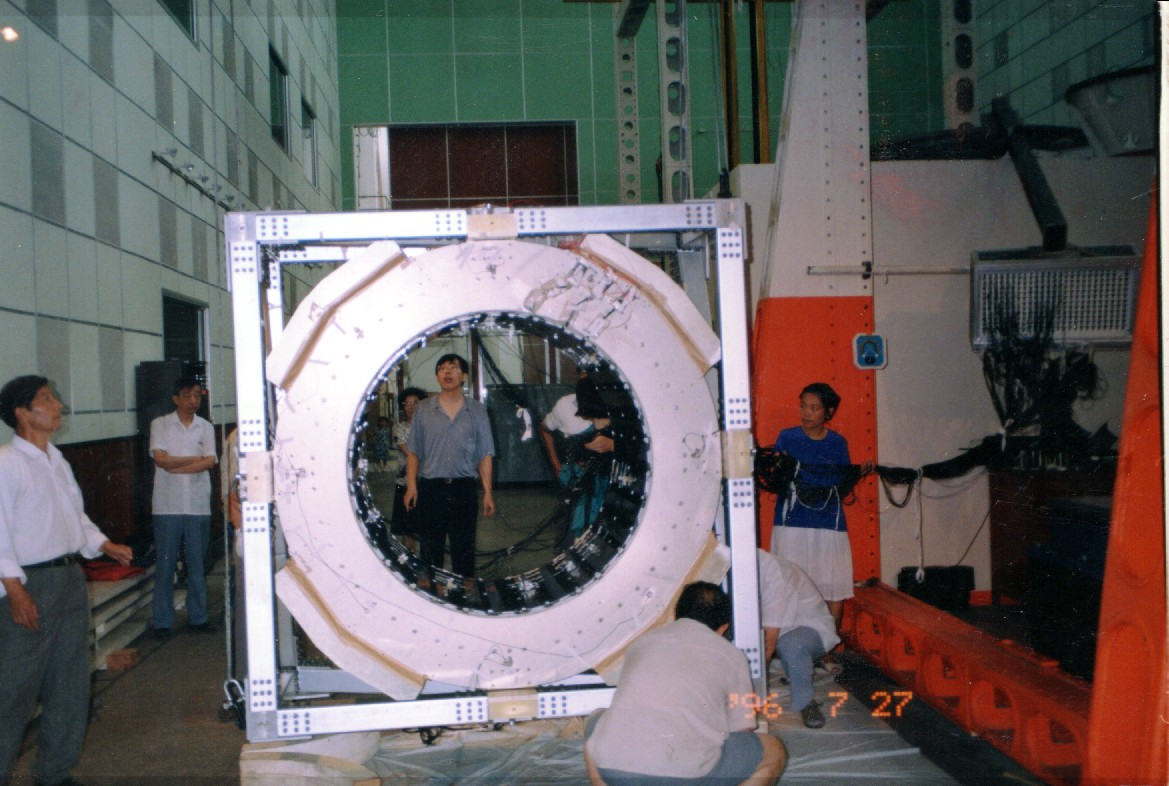
\includegraphics[width=0.8\textwidth, height=0.42\textheight ]{Figures/chapter3/Magnet/MagnetTest.jpg}
\caption[Preparing for test of the permanent magnet.]{Preparing for test of the permanent magnet in China Academy of Launch Vehicle Technology (CALT) \cite{AMSWebside}.}
\label{MagnetTest}
\end{figure}

%\begin{figure}[H]
%\centering
%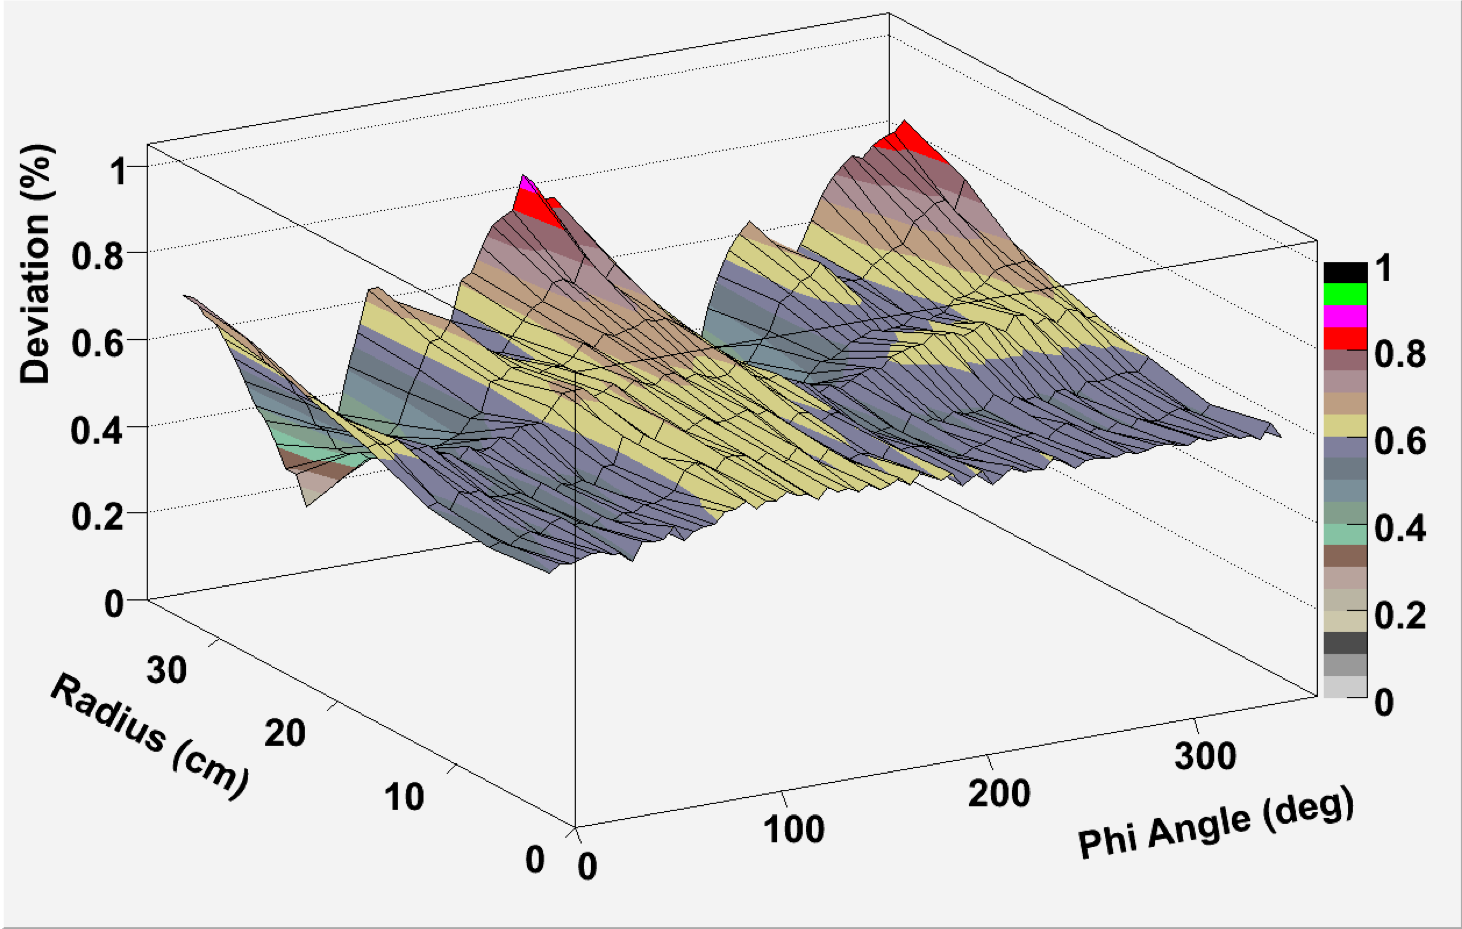
\includegraphics[width=0.8\textwidth, height=0.42\textheight ]{Figures/chapter3/Magnet/MagnetMeasurement.png}
%\caption{Deviation of the measured magnetic fields of the permanent magnet between 1997 and 2010 \cite{AMSWebside}. }
%\label{MagnetDeviation}
%\end{figure}


%%%% Tracker: With the permanent magnet, the silicon tracker can measure the charge $Z$ and also the momentum $p$ of the particle. \par
\begin{figure}[hbpt]
\centering
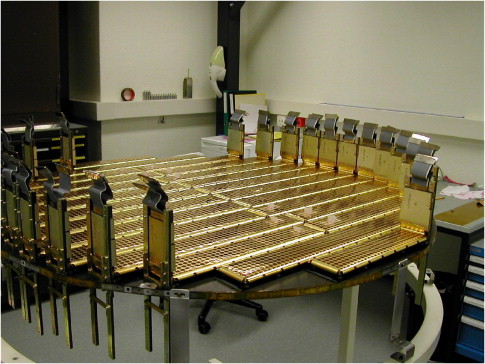
\includegraphics[width=0.8\textwidth, height=0.42\textheight ]{Figures/chapter3/Tracker/TrackerPlanePicture.jpg}
\caption[A silicon tracker inner plane fully equipped with ladders.]{A silicon tracker inner plane fully equipped with ladders \cite{TrackerPlanePicture}.}
\label{TrackerPlanePicture}
\end{figure}

%%%% Tracker Arrangement
The tracker of AMS-02 has nine silicon layers: the first layer is on the top of the TRD, the second layer is above the magnet and below the upper TOF, layers 3 to 8 are the so-called inner tracker layers as they are installed inside the permanent magnet and layer 9 is placed above the ECAL and below the RICH. In total, all nine layers have 2264 double-sided silicon micro-strip sensors. They are arranged into 192 ladders \cite{AMSTrackerPaper1, AMSTrackerPaper2}. The total active measurement area is 6.75 $m^2$. Each ladder has 1024 readout strips, 640 on the p-side and 384 on the n-side of the silicon sensors. So in total, there are 196608 readout channels. In figure \ref{TrackerPlanePicture}, a tracker inner plane equipped with ladders is shown.  \par 





%%%% Tracker Rigidity Measurement
Each double-sided silicon micro-strip sensor has a size of 41.360 $\times$ 72.045 $mm^2$ $\times$ 0.3 $mm$. When a particle goes through the sensor it creates electron-hole pairs in the middle. The created electrons drift toward the n-side and the holes toward the p-side. The X position measurement is obtained from the n-side and the Y position measurement is obtained from the p-side. Figure \ref{SiliconLayer} illustrates the process. The tracker's design results in spatial resolution of 10 $\rm{\mu m}$ and 30 $\rm{\mu m}$ in the bending and non-bending direction respectively for protons. Given the track hit positions, the rigidity and its sign can be reconstructed. By default, the rigidity is reconstructed with all the tracker layer hits. \par

\begin{figure}[htpb]
\centering
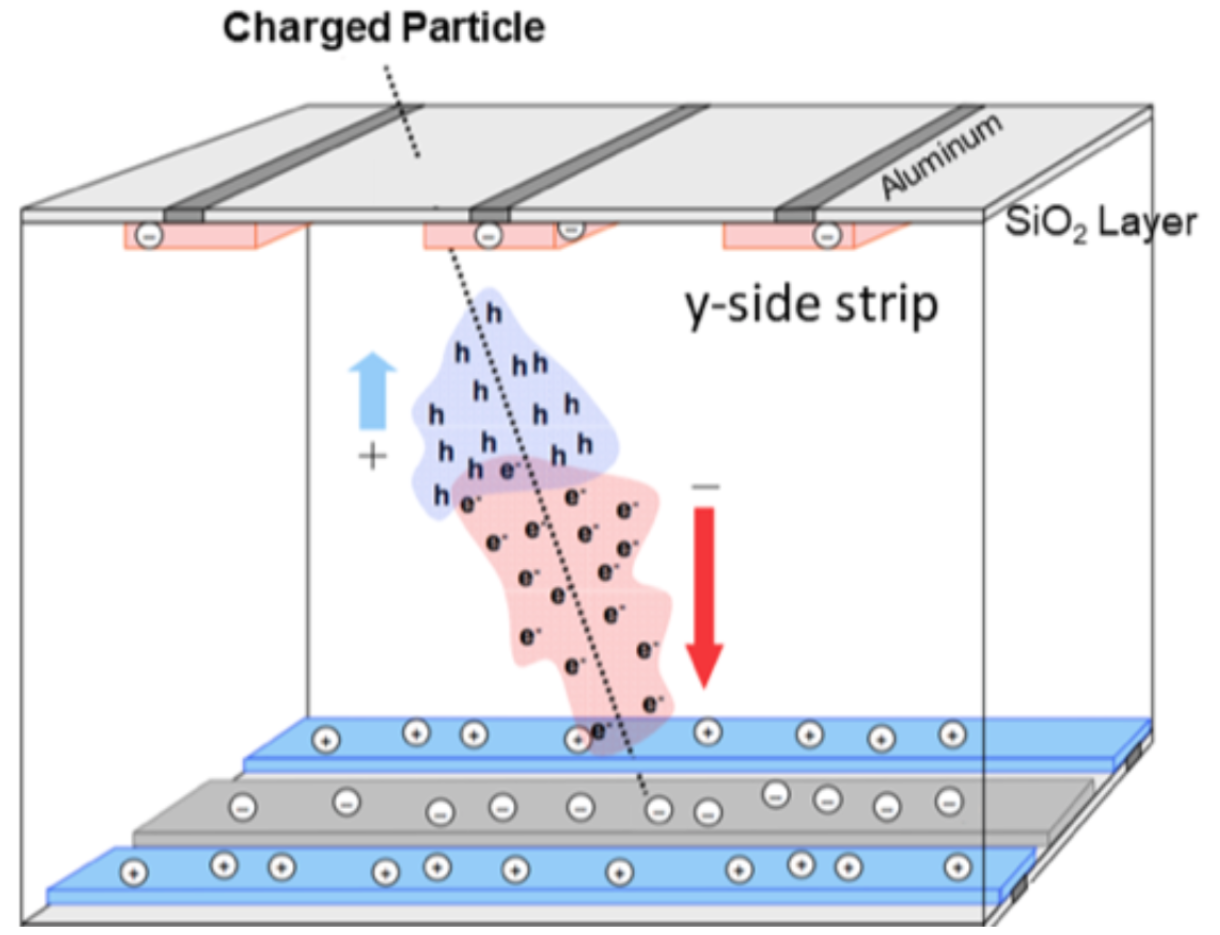
\includegraphics[width=0.8\textwidth, height=0.4\textheight ]{Figures/chapter3/Tracker/SiliconLayer.png}
\caption[Principle of operation of the double-sided silicon micro-strip sensors.]{Principle of the operation of the double-sided silicon micro-strip sensors. The electron-hole pairs produced by a charged particle drift towards the strips of the sensor as showing in this figure \cite{AMSWebside}.}
\label{SiliconLayer}
\end{figure}


%%%% Tracker Patterns
According to the presence of the tracker track hits in the different layers, various categories of tracker patterns can be defined. The tracker pattern definitions are given in table \ref{TackerPatterns}. In this table, $\checkmark$ denotes "have a hit associated to the track in this layer" and $\times$ denotes "does not have a hit associated to the track in this layer".
 
\begin{table}[h]
\center
\caption{Table of the tracker pattern definitions.}
\label{TackerPatterns}
\begin{tabular}{cccc} 
\hline
Tracker Pattern & Layer 1 & Layer 2 & Layer 9 \\
\hline
0  &  $\checkmark$   & $\checkmark$ or $\times$  & $\checkmark$   \\      %0  &  Layer 1 and 9, and maybe 2 \\
1  &  $\checkmark$   & $\checkmark$                     & $\times$            \\      %1  &  Layer 1 and 2, but not 9      \\
2  &  $\times$            & $\checkmark$                     & $\checkmark$   \\      %2  &  Layer 2 and 9, but not 1      \\
3  &  $\checkmark$   & $\times$                              &  $\times$           \\       %3  &  1 \\
4  &  $\times$            &  $\checkmark$                     &  $\times$           \\       %4  &  2 \\
5  &  $\times$           &  $\times$                              &    $\checkmark$  \\       %5  &  9 \\
-1 & $\times$            & $\times$                               & $\times$              \\       %-1 &  none \\
\hline
\end{tabular}
\end{table}


%%%% Tracker Charge Measurement
In addition, the deposited ionization energy ${\rm{d}}E/{\rm{d}}X$ is proportional to the square of the particle charge ($Z^2$). Therefore, the charge measurement in each layer can be obtained. The charge resolution of the inner tracker layers is $\Delta Z = 0.05$ for the charge of one particle.  \par



%%%% Tracker Calibration
The positions of the inner tracker layers are aligned and monitored by the Tracker Alignment System (TAS), which consists of 20 infrared laser beams that provides sub-micrometer position measurements \cite{AMSTrackerAlignment1, AMSTrackerAlignment2}. The positions of layers 1 and 9 are aligned with respect to the inner tracker by using cosmic rays over two-minute time windows. The resulting position accuracy is 5 $\rm{\mu m}$ for layer 1 and 6 $\rm{\mu m}$ for layer 9. \par 

%%%% Beam test
Before the launch of AMS-02, the whole detector was tested and calibrated at the CERN SPS  test beam facilities with 180 GeV and 400 GeV proton beams, as well as with positron, electron, and pion beams of 10 to 290 GeV. The tracker rigidity resolution function was determined with high precision and compared to MC simulation. Figure \ref{Calibration} shows the comparison between the tracker resolution measured at the 400 GeV proton beam and the one obtained by MC simulation. A good agreement between data and MC is observed.  \par

\begin{figure}[H]
\centering
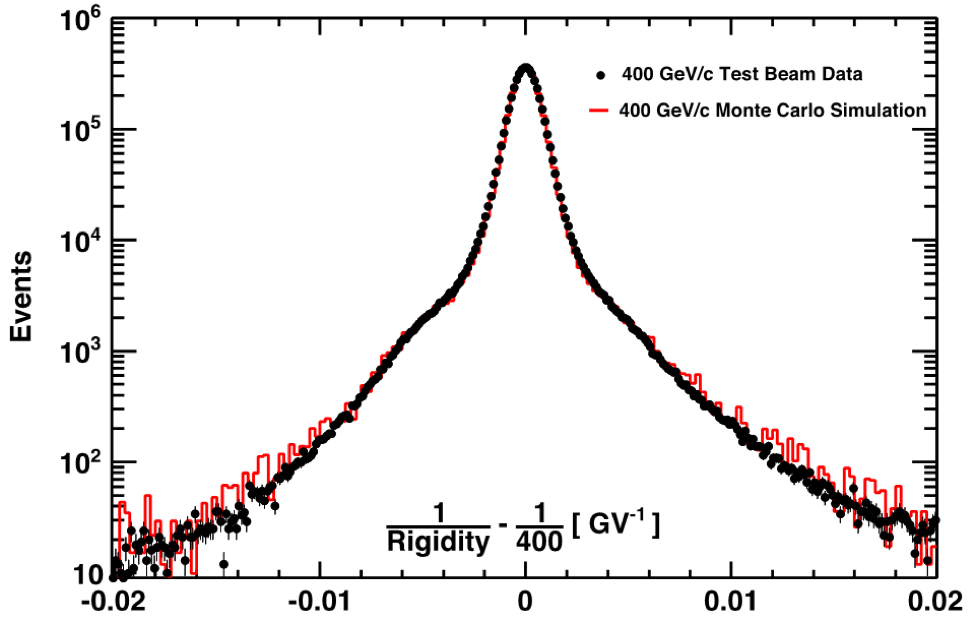
\includegraphics[width=0.8\textwidth, height=0.4\textheight ]{Figures/chapter3/Tracker/Calibration.png}
\caption[Tracker resolution measured with 400 GeV protons at the test beam and MC.]{Comparison between the tracker resolution measured with 400 GeV protons at the test beam and the MC simulation \cite{AMSWebside}.}  
\label{Calibration}
\end{figure}


%%%% Tracker Resolution 
Due to the resolution of the tracker and the multiple scattering \cite{TrackerResolutionPaper}, the resolution of the momentum measurement can be described by: 
 
\begin{equation}
\left(\frac{\sigma_{p}}{p} \right)^2 = \left( \sqrt{\frac{720}{N+4}} \frac{\sigma_{x} p  \sin \theta}{0.3 B L^2} \right)^2 + \left(\frac{0.2}{ \beta B \sqrt{LX_{0} \sin \theta} } \right)^2
\end{equation}

where $p$ is the momentum of the charged particle, $B$ is the magnetic field, $N$ is the equidistant measurements, $\theta$ is the track inclination angle, $L$ is the track length in the bending plane, $\sigma_x$ is the sagitta resolution in the bending plane, $\beta=\frac{v}{c}$, and $X_0$ is the radiation length of the traversed medium. \par 

\begin{figure}[htpb]
\centering
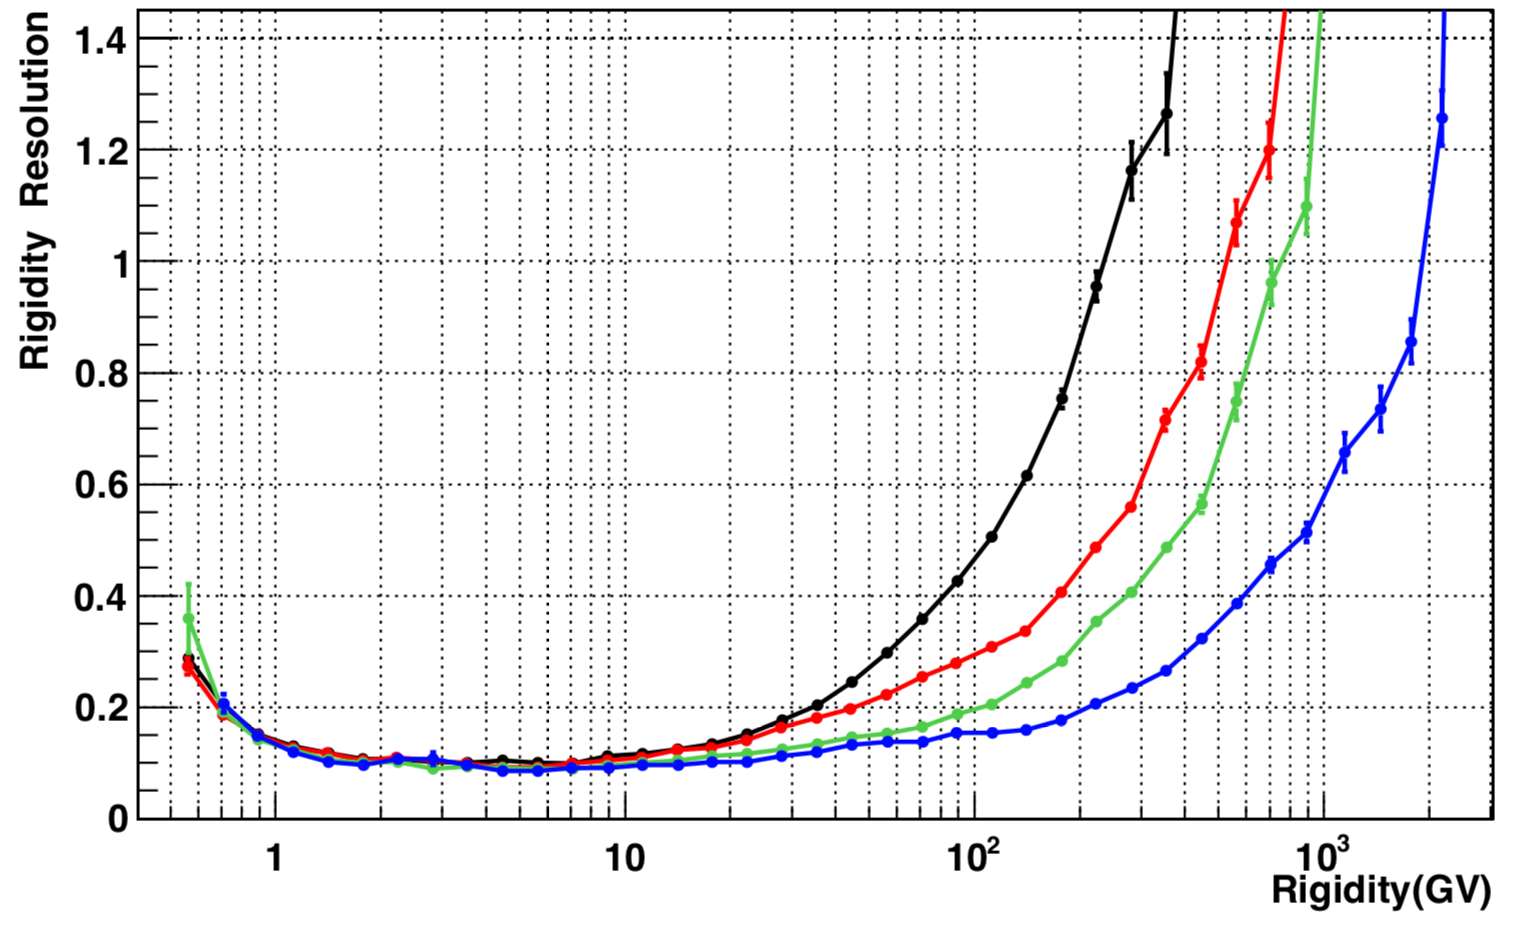
\includegraphics[width=0.9\textwidth, height=0.4\textheight ]{Figures/chapter3/Tracker/RigidityResolutionProton.png}
\caption[Tracker resolution from MC simulation for protons.]{The AMS-02 tracker resolution from MC simulation for protons \cite{ChargeConfusionReasonsAndTrackerResolutionPaper}. The four curves are for different tracker patterns: Black for inner tracker only, red for inner tracker plus layer 1, green for inner tracker plus layer 9 and blue for inner tracker plus layer 1 and 9. } 
\label{TrackerResolutions}
\end{figure}

In this equation, the momentum measurement equation consists of two terms. The first term describes the contribution of the tracker resolution and the second term the contribution of the multiple scattering. Since $R=pc/Ze$, the rigidity resolution is obtained. The AMS-02 tracker resolution has been studied extensively. In figure \ref{TrackerResolutions}, the AMS-02 simulated rigidity resolution for cosmic protons is shown. Below 1.5 GV, the rise is due to the multiple scattering, and the rise in the high rigidity range is mostly due to the detector’s resolution. The maximum detectable rigidity (MDR) is defined as the value of the rigidity $R$ where $\sigma_{R}=R$. This value is usually used to describe the highest rigidity that can be measured. For the AMS-02 tracker, the MDR for the protons in the full span (tracker pattern 0) is around 2 TV.



%\begin{figure}[h] 
%\centering   
%\subfigure[] {    
%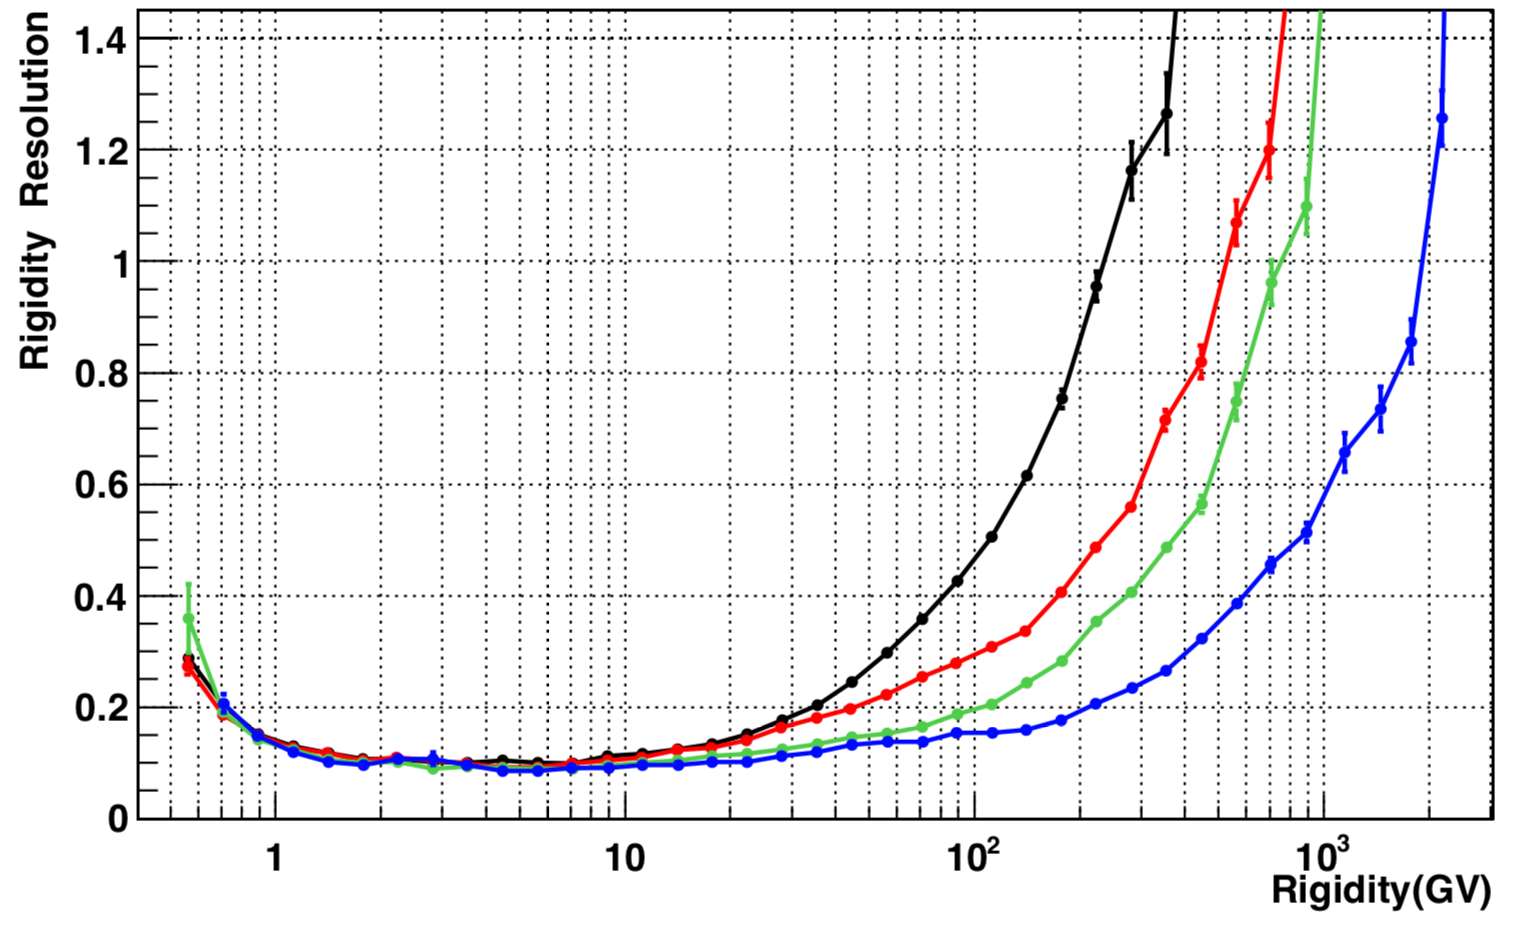
\includegraphics[width=0.45\columnwidth, height=0.225\textheight]{Figures/chapter3/Tracker/RigidityResolutionProton.png} 
%}    
%\subfigure[] { 
%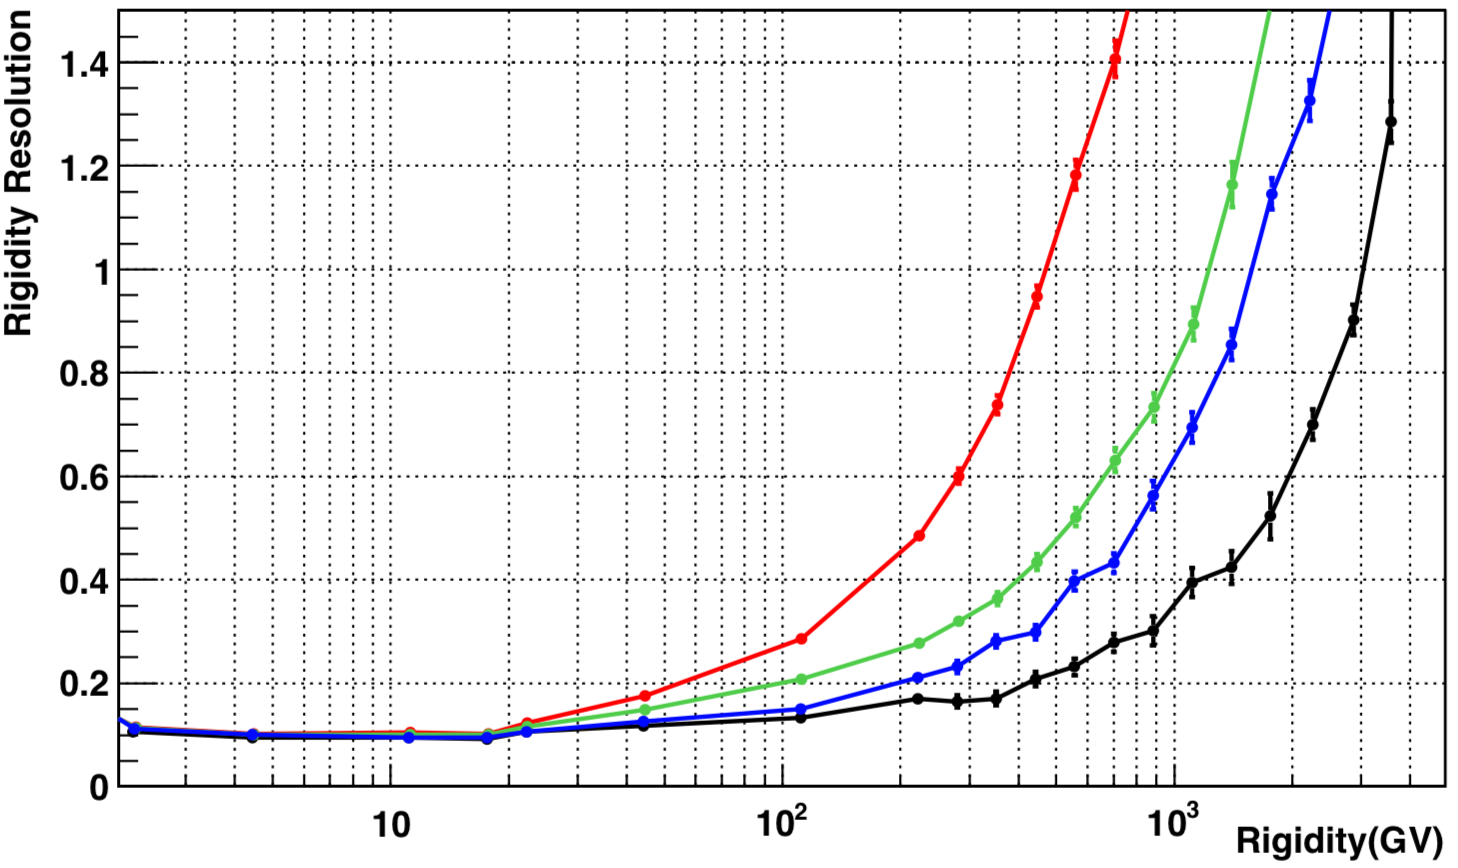
\includegraphics[width=0.45\columnwidth, height=0.225\textheight]{Figures/chapter3/Tracker/RigidityResolutionHelium.png}     
%}     
%\caption{Tracker resolution from MC simulation for a): proton and b): helium \cite{ChargeConfusionReasonsAndTrackerResolutionPaper}. The four curves are different tracker patterns: Black for inner tracker only, red for inner tracker plus layer 1, green for inner tracker plus layer 9, blue for inner tracker plus layer 1 and 9. } 
%\label{TrackerResolutions}    
%\end{figure}


%-----------------------------------------------------------------------------------------------------------------
%%%% TTCS off 
The heat produced by the electronics and radiators of the tracker can be removed by the Tracker Thermal Cooling System (TTCS). The TTCS is a two-phase $\rm{CO_2}$ cooling system with four cooling pumps. Due to aging and technique problems, the old four pumps were replaced by four new pumps in several spacewalks from November 2019 to January 2020.  




